\chapter{The Nature And Eradication Of Fear}

This chapter follows J. Krishnamurti's San Diego conversation with Dr. Alan W. Anderson on fear. There are no validated blackboard images or equations for this lecture, so the mathematical structure below is deliberately schematic: it is a disciplined notation for the movement of the inquiry, not a formal psychological or physical model. The source remains the spoken investigation: fear is first seen in its many forms, then questioned at its root, and finally related to thought, knowledge, intelligence, and freedom.

\section{The Whole Movement Of Fear}

The conversation resumes where the previous one had left off: the question of fear has appeared, and now it must be explored carefully. Krishnamurti does not begin with a definition. He begins with range. Fear may be fear of death, fear of loneliness, fear of not being loved, fear of failure, fear of not becoming successful, fear of losing physical security. The first point is that fear is not a private oddity. It is a common human fact.

He also warns that fear cannot finally be separated from pleasure. They are named as two sides of the same coin, though pleasure is not yet unfolded in this conversation. In a compact notation, we may write only this much:

\begin{equation}
\text{fear} \leftrightarrow \text{pleasure}.
\end{equation}

This is not an equation in the scientific sense. It marks a paired movement in the inquiry. The lecture will first take up fear, but it leaves a bridge to pleasure.

Krishnamurti then proposes the order of investigation. We begin with outward, physical fears and move inward. That order matters. If we begin with the abstract question ``What is fear?'' too soon, we may answer with a theory. If we begin with what human beings actually fear, the question gathers force.

Let \(F\) denote, only schematically, the whole field or movement of fear. Then the lecture first separates two regions, while later insisting that they are deeply interrelated:

\begin{equation}
F = F_{\mathrm{physical}} \cup F_{\mathrm{psychological}}.
\end{equation}

Here \(F_{\mathrm{physical}}\) includes fears bound up with food, shelter, work, pain, survival, and death. \(F_{\mathrm{psychological}}\) includes fear of loneliness, dependence, rejection, not being, public opinion, image, and spiritual or worldly failure. The union sign is useful, but it should not mislead us. Krishnamurti's point is not that these are sealed compartments. The outer and the inner keep entering one another.

\section{Physical Security And The Disorder Of Division}

The first serious step is physical security. The brain, Krishnamurti says, needs security as a child needs security. Without it, action becomes distorted, unhealthy, lopsided. Food, clothing, and shelter are not luxuries; they are necessary conditions for sane human functioning.

But the inquiry immediately turns paradoxical. Human beings need security, yet the structures they build in the name of security often destroy it. Nations divide themselves as Americans, Russians, Indians, Chinese. Governments arm themselves. Competition hardens. Occupation becomes a source of fear because a job depends on systems of production, trade, consumerism, and competition among countries. The mind wants security and yet acts in ways that deny security.

A schematic form of the contradiction is:

\begin{align}
\text{brain} &\longrightarrow \text{needs security}, \\
\text{division} + \text{competition} + \text{war} &\longrightarrow \text{destruction of security}.
\end{align}

So the first movement of the lecture is not simply social criticism. It is a structural observation. We ask for security while maintaining disorder. This disorder is not outside us as a distant political fact; it is continuous with the mind that separates, identifies, competes, and protects its own image.

The concrete examples keep the inquiry grounded. The fear of losing a job, the fear of hunger, the sight of poverty, the burden of plans that become more important than starvation itself: these are not illustrations added after the theory. They are the route by which the inquiry moves inward.

\section{Outer Fear Becomes Inner Fear}

The next transition is pain. One has had physical pain, perhaps last week, and the mind fears that it may return. Anderson observes that what is remembered is not merely the neurological event but the emotion attending it. Krishnamurti accepts the point and continues. Fear has begun to show its relation to memory and time.

A small worked example is enough:

\begin{enumerate}
\item A physical pain occurs.
\item Memory carries the emotional mark of that pain.
\item Thought projects recurrence: it may happen again.
\item The projected recurrence is experienced now as fear.
\end{enumerate}

In schematic form:

\begin{equation}
\text{pain}_{\mathrm{past}} + \text{memory} + \text{projection into tomorrow}
\longrightarrow
\text{fear now}.
\end{equation}

The notation is useful because it shows the movement without pretending to measure it. Fear is not just the pain. It is the remembered pain carried by thought into possible recurrence.

From pain, Krishnamurti moves to public opinion, reputation, and image. What will the neighbour say? What will society think? If I live in a particular religious or social environment, I may outwardly conform because my job, status, or respectability depends on it. Public opinion becomes another form of fear.

The outward and inward are now inseparable. A job is outward; the image of respectability is inward. Poverty is outward; the hopelessness around poverty enters the human mind. Public opinion is outward; dependence on that opinion is inward. The lecture does not yet name thought as the root, but it is preparing the ground.

\section{Dependency, Loneliness, And Identification}

The conversation now moves into the more complicated inward fears. Dependency is central. I depend on my wife, my husband, my guru, my priest, my belief, my country, my image. If the person turns away, if the belief fails, if the image cracks, I am frightened. I may become jealous, violent, anxious, or defensive, because what I called relationship was partly dependence.

Loneliness then becomes a major factor. To avoid loneliness, one may attach oneself to another person, a belief, a saviour, a guru, or an ideology. Anderson describes this as filling the hole with a new image. Krishnamurti rejects the image as another form of disorder. The attachment does not end fear; it protects and extends it.

We may summarize this movement as:

\begin{equation}
\text{loneliness} \longrightarrow \text{attachment} \longrightarrow \text{dependence} \longrightarrow \text{fear of loss}.
\end{equation}

The same structure appears in achievement. One fears not arriving, not succeeding, not becoming enlightened, not expanding consciousness, not being somebody. The fear of not being translates itself into identification: with country, with God, with an invented image of oneself. Krishnamurti's reversal is sharp: man has not merely received an image from heaven; man has made God in his own image.

At this point the list of fears is long: logical fears, irrational fears, neurotic fears, survival fears, hidden fears. The accumulation is important. It creates the need for the next question.

\subsection{Question \& Answer}

\paragraph{Question.}
Can we deal with fear one by one? Can we take loneliness, then public opinion, then pain, then death, then dependency, and solve each fear separately?

\paragraph{Answer.}
Krishnamurti's answer is no. To take one branch after another is to spend a lifetime pruning leaves while the root remains untouched. Anderson names the danger: we would be caught in fragmentation. Krishnamurti adds that analysis itself becomes paralysis. If I analyse fear, I may then fear that I have not analysed correctly; I may seek another analyst; the process continues.

The branch-by-branch method can be written as a failed rule:

\begin{equation}
\{f_1,f_2,\ldots,f_n\}
\longrightarrow
\text{fragmented analysis}
\longrightarrow
\text{paralysis}.
\end{equation}

The alternative is not a quicker analysis. It is a different question:

\begin{equation}
\text{many fears}
\longrightarrow
\text{the whole movement of fear}
\longrightarrow
\text{root inquiry}.
\end{equation}

This is one of the central turns of the lecture. We stop asking how to manage the branches and ask what fear is.

\begin{figure}
\centering
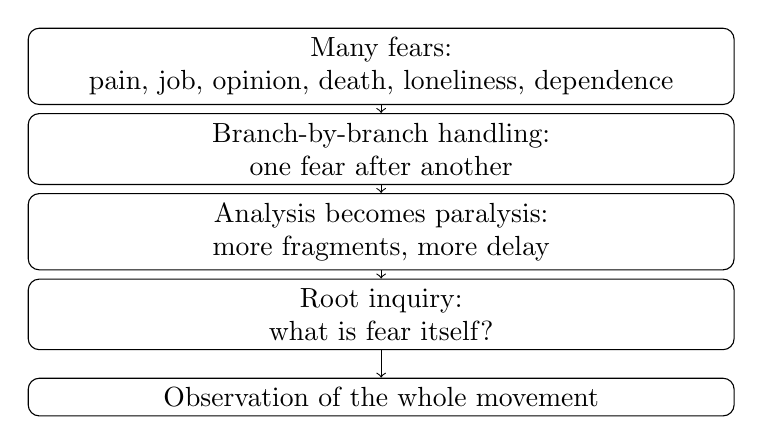
\begin{tikzpicture}[node distance=1.05cm]
\node[draw, rounded corners, align=center, text width=0.72\linewidth] (many) {Many fears:\\ pain, job, opinion, death, loneliness, dependence};
\node[draw, rounded corners, align=center, text width=0.72\linewidth, below of=many] (branch) {Branch-by-branch handling:\\ one fear after another};
\node[draw, rounded corners, align=center, text width=0.72\linewidth, below of=branch] (paralysis) {Analysis becomes paralysis:\\ more fragments, more delay};
\node[draw, rounded corners, align=center, text width=0.72\linewidth, below of=paralysis] (root) {Root inquiry:\\ what is fear itself?};
\node[draw, rounded corners, align=center, text width=0.72\linewidth, below of=root] (observe) {Observation of the whole movement};
\draw[->] (many) -- (branch);
\draw[->] (branch) -- (paralysis);
\draw[->] (paralysis) -- (root);
\draw[->] (root) -- (observe);
\end{tikzpicture}
\end{figure}

\section{What Is Fear When Escape Ends?}

Krishnamurti now refuses description. Fear is not to be found by naming its objects or repeating explanations. What is fear behind words, behind description, behind escape, behind analysis? Anderson notices that his own academic response is inadequate. To say, ``if I have followed you,'' and then produce a description is already to move away from the fact. Fear has to be discovered directly, as hunger is discovered directly.

Here the lecture's rhythm slows. Krishnamurti says: I am not escaping; I am not rationalizing; I am not analysing. No backing off, no flight, no explanation. The movement is negative, but not nihilistic. Negation clears the field.

There is also the problem of hidden fear. Can the conscious mind invite hidden fears to the surface? Krishnamurti says the conscious can deal with what it knows, but it cannot observe what it does not know. Dreams are mentioned and set aside as a continuation of daily movement in another form. The real question is how hidden fears can be exposed naturally, so that the mind sees them completely.

Anderson then makes the dialogue itself an example. In a university setting, one may listen while silently preparing a response, guarding reputation, worrying about whether one appears intelligent. Fear prevents listening. The professor's image is at stake. Thus the abstract question of hidden fear becomes immediate: the fear is operating in the very act of conversation.

\subsection{Question \& Answer}

\paragraph{Question.}
If conscious analysis cannot expose hidden fear, and escape is futile, what action remains?

\paragraph{Answer.}
Krishnamurti's answer begins with negation. Escape, analysis, rationalization, resistance, and identification are seen as futile. When these dissipating movements end, there is energy. This energy is not physical energy and not mystical spectacle. It is the gathered energy of attention when the usual leaks have stopped.

The schematic relation is:

\begin{equation}
\neg(\text{escape}+\text{analysis}+\text{identification}+\text{resistance})
\longrightarrow
\text{undissipated energy}.
\end{equation}

But here Krishnamurti makes another crucial move. When faced with fear, we ask, ``What can I do?'' He answers: I cannot do anything. Why? Because the ``I'' that wants to act is implicated in the production of fear. Public opinion, image, dependency, identification -- these are not external objects accidentally attached to the self. They are part of the self's movement.

So the question changes again. Not: what shall I do to fear? But: what has brought fear about?

\section{Thought, Recognition, And The Observer}

The inquiry now becomes exact. What has created fear? My neighbour? My country? My culture? Myself? Krishnamurti presses the question but does not settle for an academic answer. The answer must be seen, not adopted.

The next step is observation. Can the mind observe fear, not one piece of fear, not a succession of fears, but the whole movement of fear? Can it observe without the thought that has created the observer?

We may write the central identity of this part schematically:

\begin{equation}
\text{observer} = \text{thought}.
\end{equation}

This is not a metaphysical formula. It is a way of preserving the lecture's claim: the observer who says ``I am afraid'' is not separate from the movement of thought that names, recognizes, remembers, and projects fear.

The process can be represented as follows:

\begin{align}
\text{previous experience} &\longrightarrow \text{recognition}, \\
\text{recognition} &\longrightarrow \text{naming: ``fear''}, \\
\text{naming} + \text{memory} &\longrightarrow \text{projection}, \\
\text{projection} &\longrightarrow \text{fear sustained}.
\end{align}

Krishnamurti's examples remain concrete. I am afraid of what my neighbour says because I want respectability. Thought has divided the world into nations and thereby destroyed physical security. I am lonely, and thought acts neurotically to escape loneliness. I had pain yesterday, and thought projects it into tomorrow. In each case, thought nourishes fear.

The interesting turn is his statement that fear is new each time, and made old by recognition. Recognition belongs to knowledge, to the past. When the mind names the present fact by association with what has been, it gives continuity to fear.

The ending is stated very simply:

\begin{equation}
\text{observation without the observer}
\longrightarrow
\text{fear is not}.
\end{equation}

We should not turn this into a technique. It is not a method to practise in order to get a result. In the lecture, it follows from seeing the whole movement of fear and the whole movement of thought.

\begin{figure}
\centering
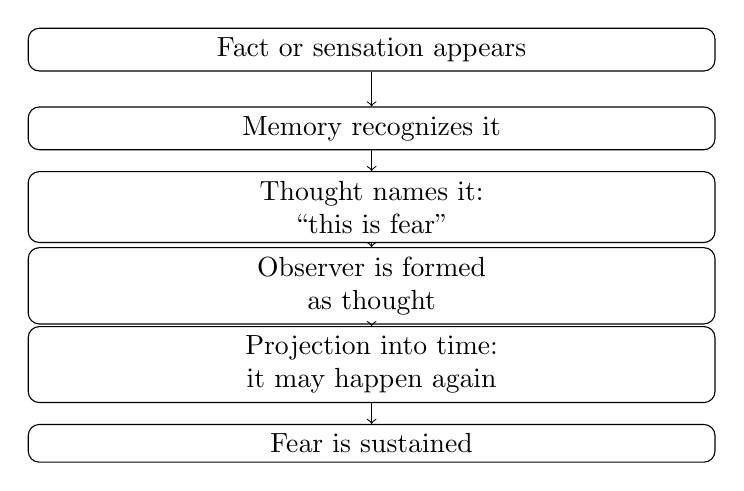
\begin{tikzpicture}[node distance=1.0cm]
\node[draw, rounded corners, align=center, text width=0.70\linewidth] (fact) {Fact or sensation appears};
\node[draw, rounded corners, align=center, text width=0.70\linewidth, below of=fact] (memory) {Memory recognizes it};
\node[draw, rounded corners, align=center, text width=0.70\linewidth, below of=memory] (name) {Thought names it:\\ ``this is fear''};
\node[draw, rounded corners, align=center, text width=0.70\linewidth, below of=name] (observer) {Observer is formed\\ as thought};
\node[draw, rounded corners, align=center, text width=0.70\linewidth, below of=observer] (projection) {Projection into time:\\ it may happen again};
\node[draw, rounded corners, align=center, text width=0.70\linewidth, below of=projection] (sustain) {Fear is sustained};
\draw[->] (fact) -- (memory);
\draw[->] (memory) -- (name);
\draw[->] (name) -- (observer);
\draw[->] (observer) -- (projection);
\draw[->] (projection) -- (sustain);
\end{tikzpicture}
\end{figure}

\section{Intelligence, Knowledge, And Freedom}

Krishnamurti then protects the inquiry from a misunderstanding. If a bus rushes toward us, or if we see a dangerous animal, we move. That is not psychological fear in the sense being examined. It is intelligent self-protection. It is intelligence operating.

\begin{table}
\centering
\begin{tabular}{p{0.43\linewidth}p{0.43\linewidth}}
\textbf{Self-protective intelligence} & \textbf{Psychological fear} \\
Stepping away from a rushing bus & Fear of public opinion \\
Moving away from immediate danger & Fear of recurring pain through memory \\
Direct response to fact & Loneliness sustained by image and attachment \\
No need for inner narrative & Thought projecting past into future \\
\end{tabular}
\end{table}

This distinction is essential. The lecture is not asking human beings to ignore danger. It is asking whether the other movement -- the movement of thought, image, recognition, and projection -- can end.

Krishnamurti then asks whether thought can understand itself, know its place, and not project itself. Control is rejected. If thought controls thought, the controller is another fragment of thought. That game has no end.

A final worked derivation can be put this way:

\begin{enumerate}
\item Thought has a practical field: language, driving, science, mathematics, ordinary skill.
\item Thought also carries psychological accumulation: image, tradition, respectability, fear of what has been and what may be.
\item When psychological accumulation tries to understand fear, it turns the living fact into something old.
\item To understand what is, accumulated psychological knowledge has no transforming power.
\item Therefore freedom from fear is not produced by knowledge.
\end{enumerate}

The notation is:

\begin{align}
K_{\mathrm{practical}} &\neq K_{\mathrm{psychological}}, \\
K_{\mathrm{psychological}} &\not\Rightarrow \text{freedom from fear}.
\end{align}

This is close to the lecture's final turn. Knowledge is necessary in its proper place. Speaking a language, driving, science, mathematics -- these require knowledge. But when we ask about the transformation of fear, the accumulated knowledge of experience, tradition, respectability, and image has no value. It may even become ignorance.

Krishnamurti closes by saying that freedom is not born of knowledge. Freedom is not something to be searched for as another object. It comes when the burden is not.

\begin{equation}
\text{freedom} \notin K,
\qquad
\text{freedom appears when burdens are absent}.
\end{equation}

The language must remain careful here. Nothing new is put in the place of fear as a compensating idea. The chapter should not turn the ending into a promise or a method. The spoken movement is simpler and more austere: when thought, as observer, no longer sustains fear, fear is not.

\section{Summary}

The lecture moves from many fears to the whole movement of fear. It begins with physical security and shows how human division destroys what the brain needs. It passes through pain, public opinion, death, poverty, dependency, loneliness, achievement, and identification until the list itself becomes impossible to handle one item at a time.

That impossibility produces the root question. Analysis of fragments is paralysis. Escape, rationalization, identification, and resistance dissipate energy. When they are seen as futile, the mind has energy to ask what has brought fear about.

The answer is not a definition but a seeing: thought, through memory, recognition, naming, projection, and the observer, sustains psychological fear. Intelligent self-protection is different; it acts directly in danger. Practical knowledge has its proper place, but accumulated psychological knowledge cannot transform fear. Freedom is not born of knowledge. It is present when the burden that thought carries is no longer there.